\section{Debugger}

Die Debugger-""Komponente vermittelt zwischen dem Debug-""Modell der GUI-""Plattform und dem Interpreter. Außerdem ist in dieser Komponente die Funktionalität zum Starten des Interpreters aus der GUI (Launching) enthalten.

\subsection{Debugging}

Dieser Teil des Debuggers implementiert das Debug-""Modell von Eclipse. Somit können alle in Eclipse vorhandenen Debug-""Ansichten (etwa Breakpoint-""Manager, Variablenansicht, Ausdrucksansicht) mit dem Worthwhile-""Interpreter kommunizieren.

Eine Übersicht über dieses Modell findet sich in Abbildung~\ref{debugmodel}.

\begin{figure}
	\caption[B]{Das Debug-""Modell von Eclipse und dessen Implementierung\footnotemark}
	\centering
	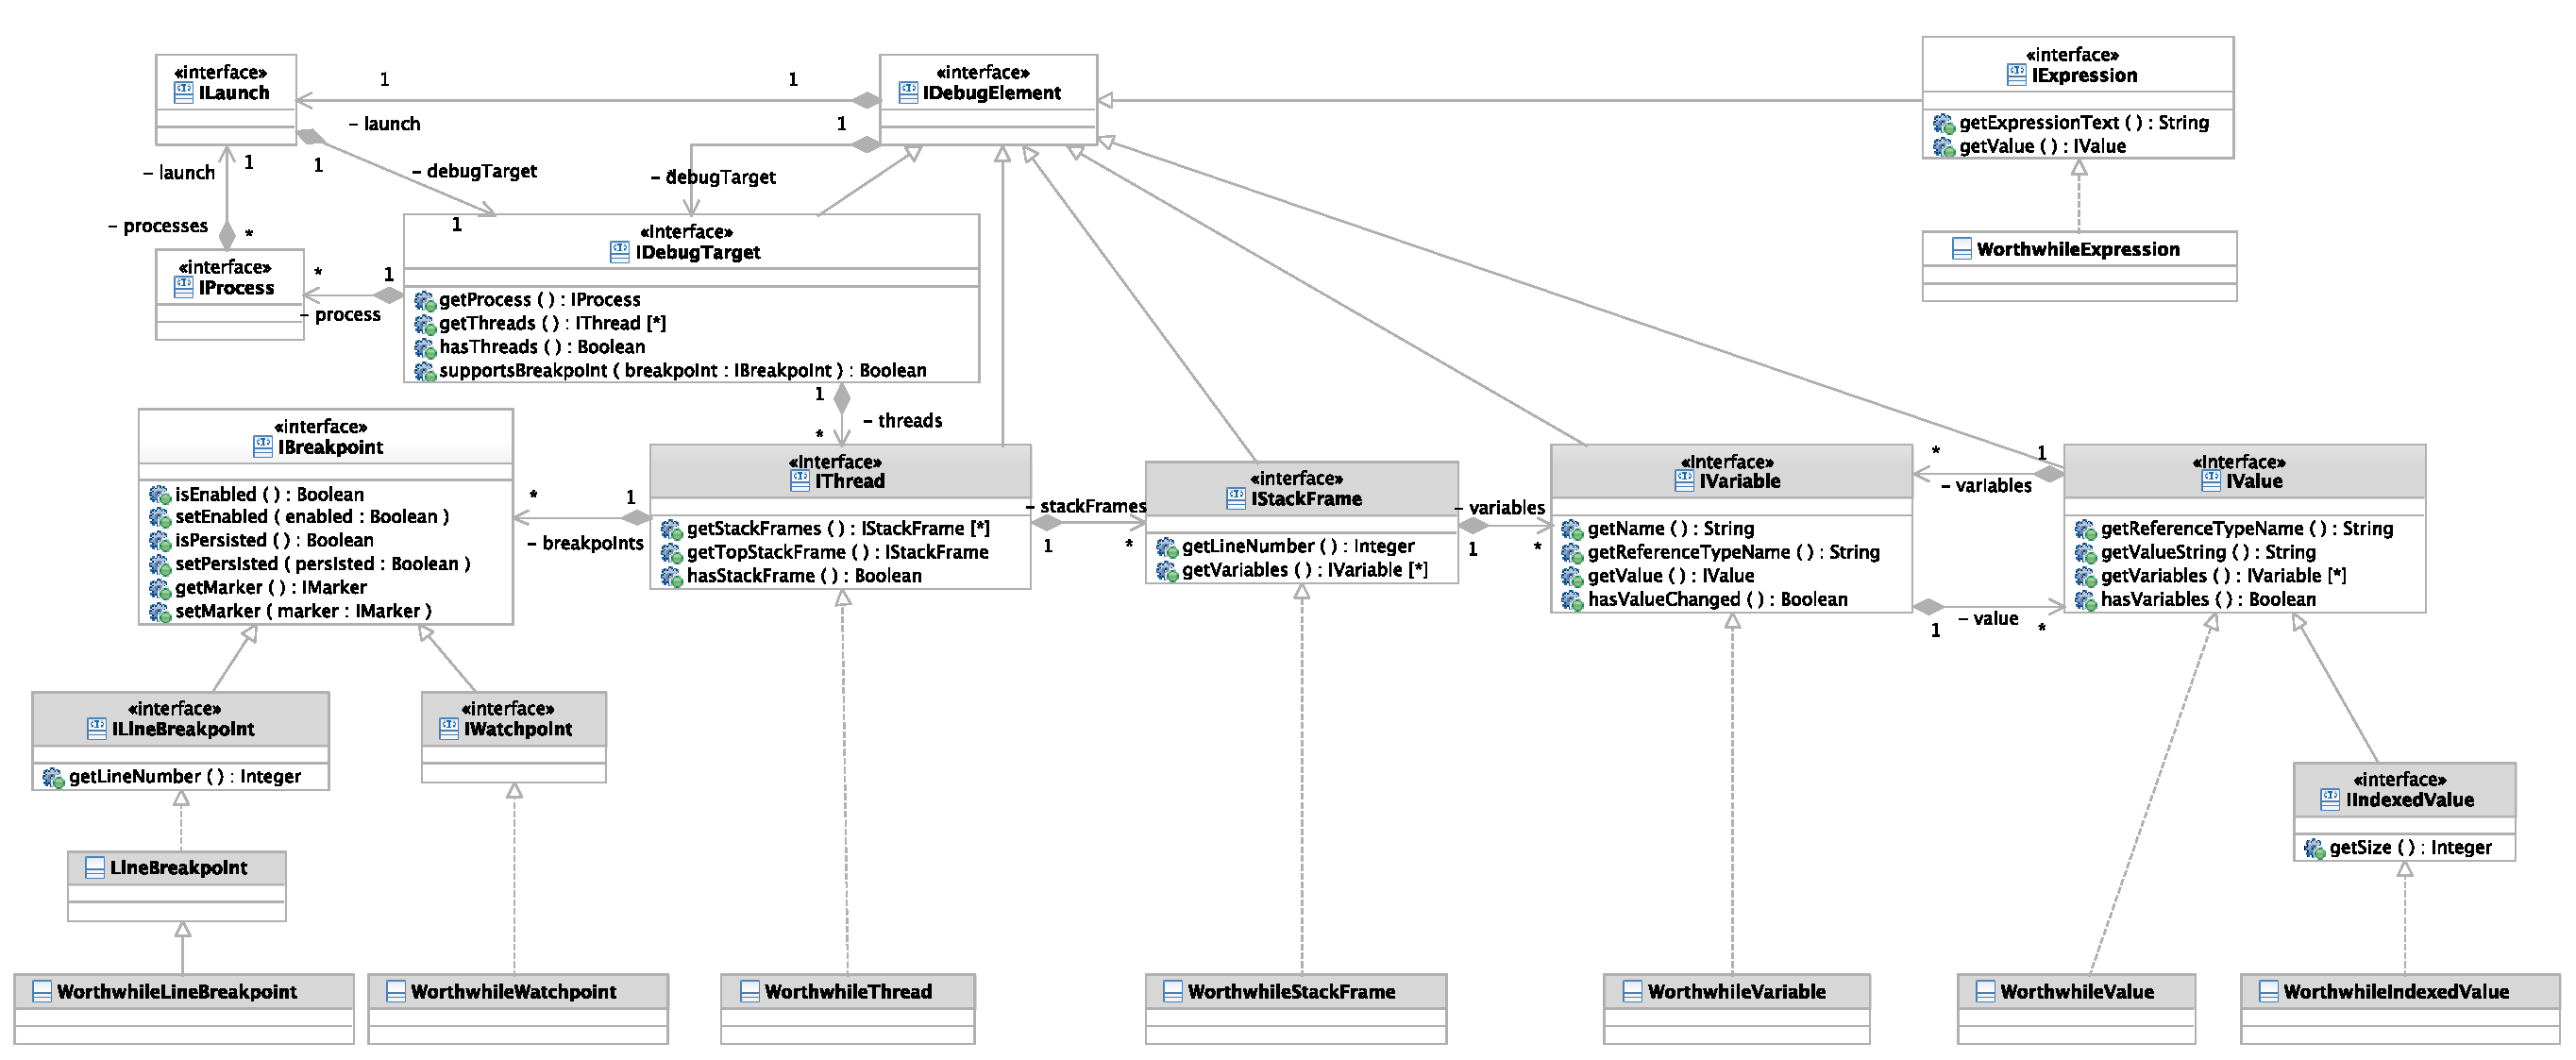
\includegraphics[angle=90,height=\textheight]{diagrams/debugmodel.pdf}
	\label{debugmodel}
\end{figure}
\footnotetext{basierend auf \url{http://www.eclipse.org/articles/Article-Debugger/how-to.html}}

\subsubsection{class WorthwhileDebugTarget}

Diese Klasse stellt die Schnittstelle zwischen GUI und Interpreter bereit. Sie übernimmt die Kommandos von der GUI und übersetzt sie in Kommandos für den Interpreter (bzw.\ dessen \texttt{DebugInterface}).

\begin{description}
	\method{public IProcess getProcess()} Gibt den Prozess zurück, der den Interpreter ausführt.
	\method{public IThread[] getThreads()} Gibt eine Liste der Threads zurück, die zu diesem Interpreterlauf gehören.
	\method{public boolean hasThreads()} Gibt an, ob momentan irgendwelche Threads vorhanden sind.
	\method{public boolean supportsBreakpoint(IBreakpoint breakpoint)} Gibt an, ob das Setzen des angegebenen Breakpoints unterstützt wird.
\end{description}

\subsubsection{class WorthwhileThread}

Ein Thread repräsentiert einen sequentiellen Programmablauf. Da die WHILE-""Sprache kein Multithreading unterstützt, gibt es für jeden Interpreterlauf nur eine Instanz dieser Klasse. Ein Thread ermöglicht den Zugriff auf \texttt{StackFrames}, wenn die Programmausführung pausiert ist.

\begin{description}
	\method{public IStackFrame[] getStackFrames()} Gibt alle in diesem Thread enthaltenen Stackframes zurück.
	\method{public IStackFrame getTopStackFrame()} Gibt den obersten Stackframe zurück.
	\method{public boolean hasStackFrame()} Gibt zurück, ob der Thread im Moment Stackframes besitzt.
\end{description}

\subsubsection{class WorthwhileStackFrame}

Ein Stackframe repräsentiert in der GUI einen Ausführungskontext eines Programms. Dazu gehören insbesondere die an der aktuellen Ausführungsposition sichtbaren Variablen.

\begin{description}
	\method{public int getLineNumber()} Gibt die Zeilennummer der Ausführungsposition in der Quelldatei zurück.
	\method{public IVariable[] getVariables()} Gibt die im Ausführungskontext sichtbaren Variablen zurück.
\end{description}

\subsubsection{class WorthwhileVariable}

Diese Klasse repräsentiert eine Variable in einem Ausführungskontext. Jede Variable besitzt einen Typ und einen veränderbaren Wert.

\begin{description}
	\method{public String getName()} Gibt den Namen der Variablen zurück.
	\method{public String getReferenceTypeName()} Gibt eine textuelle Repräsentation des Datentyps der Variablen zurück.
	\method{public IValue getValue()} Gibt den Wert der Variablen zurück.
	\method{public boolean supportsValueModification()} Gibt an, ob der Wert dieser Variablen verändert werden kann.
	\method{public void setValue(IValue value)} Setzt den Wert dieser Variablen auf den angegebenen Wert.
	\method{public void setValue(String expression)} Setzt den Wert dieser Variablen auf den Wert des übergebenen Ausdrucks.
	\method{public void verifyValue(IValue value)} Prüft, ob der angegebene Wert als neuer Wert für diese Variable gesetzt werden kann.
	\method{public void verifyValue(String expression)} Prüft, ob das Ergebnis des angegebenen Ausdrucks als neuer Wert für diese Variable gesetzt werden kann
	\method{public boolean hasValueChanged()} Gibt an, ob sich der Wert der Variablen seit der letzten Pausierung des Programmablaufs geändert hat.
\end{description}

\subsubsection{class WorthwhileValue}

Diese Klasse repräsentiert den Wert einer Variablen.

\begin{description}
	\method{public String getReferenceTypeName()} Gibt eine textuelle Repräsentation des Datentyps des Wertes zurück.
	\method{public String getValueString()} Gibt eine textuelle Repräsentation des Wertes zurück.
	\method{public IVariable[] getVariables()} Gibt eine Liste aller enthaltenen Variablen (z.~B.\ Werte in einem Array) zurück.
	\method{public boolean hasVariables()} Gibt zurück, ob dieser Wert enthaltene Variablen besitzt.
\end{description}

\subsubsection{class WorthwhileExpression}

Diese Klasse repräsentiert einen auszuwertenden benutzerdefinierten Ausdruck.

\begin{description}
	\method{public String getExpressionText()} Gibt den Quellcode des Ausdrucks zurück.
	\method{public IValue getValue()} Gibt den aktuellen Wert des Ausdrucks zurück.
\end{description}

\subsubsection{class WorthwhileLineBreakpoint}

Diese Klasse repräsentiert einen Breakpoint, der an eine bestimmte Zeile im Programmtext gebunden ist und die Programmausführung anhält, sobald diese Zeile erreicht wird.

\begin{description}
	\method{public int getLineNumber()} Gibt die Zeilennummer dieses Breakpoints zurück.
	\method{public IMarker setMarker()} Setzt die Markierung, die diesem Breakpoint zugeordnet ist. Diese Markierung enthält alle notwendigen Informationen zum Breakpoint und wird auch über das Ende einer GUI-""Sitzung hinaus gespeichert.
\end{description}

\subsubsection{class WorthwhileWatchpoint}

Diese Klasse repräsentiert einen \textit{Watchpoint}, also einen Breakpoint, der an eine Variable gebunden ist und die Programmausführung anhält, sobald ihr Wert gelesen oder verändert wird.

\begin{description}
	\method{public IMarker setMarker()} Setzt die Markierung, die diesem Watchpoint zugeordnet ist. Diese Markierung enthält alle notwendigen Informationen zum Watchpoint und wird auch über das Ende einer GUI-""Sitzung hinaus gespeichert.
\end{description}

\subsection{Launching}

\subsubsection{class WorthwhileLaunchDelegate}

Der \texttt{LaunchDelegate} ist dafür verantwortlich, den Interpreter zu starten und zu initialisieren sowie die Verbindung zwischen Interpreter und Debug-""Infrastruktur herzustellen.

\begin{description}
	\mlmethod{public void launch(ILaunchConfiguration~configuration, String~mode, ILaunch~launch, IProgressMonitor~monitor)}
	Diese Methode wird von der GUI aufgerufen, wenn der Benutzer den Befehl zum Ausführen des Programms wählt. Dabei enthält \texttt{configuration} die nötigen Einstellungen zum Aufruf des Interpreters, etwa den Pfad zur ausführbaren Datei von Z3 oder Optionen für den Interpreter. \texttt{mode} enthält den Modus, in dem das Programm ausgeführt wird, und ist entweder \texttt{run} oder \texttt{debug}. Der Parameter \texttt{launch} enthält Informationen über diese Ausführung des Programms; die Aufgabe der \texttt{launch()}-Methode ist es, sämtliche erzeugten Prozesse und \texttt{DebugTarget}s diesem Objekt bekannt zu machen. Schließlich kann der Fortschritt der Ausführung dem Benutzer über das \texttt{monitor}-""Objekt mitgeteilt werden.
\end{description}

\subsubsection{class WorthwhileSourcePathComputerDelegate}

Diese Klasse ist dafür verantwortlich, die Pfade zu bestimmen, die auf der Suche nach Quelldateien (Source Lookup) durchsucht werden sollen. Ein Source Lookup wird immer dann nötig, wenn der aktuelle Ausführungszustand des Interpreters auf die Quelldatei zurückgeführt werden soll, etwa bei der Anzeige der aktuell ausgeführten Zeile.

\begin{description}
	\mlmethod{public ISourceContainer[] computeSourceContainers( ILaunchConfiguration~configuration, IProgressMonitor~monitor)}
	Ruft eine Liste aller Pfade ab, die beim Source Lookup nach Quelldateien durchsucht werden.
\end{description}

\subsubsection{class WorthwhileSourceLookupParticipant}

Für den Source Lookup kann sich eine Reihe von Klassen (Participants) registrieren, die ein Objekt einer Quelldatei zuordnen. Ein solcher Participant wird in dieser Klasse implementiert.

\begin{description}
	\method{public String getSourceName(Object object)} Ruft den Quelldateinamen für \texttt{object} ab, wenn es sich dabei um eine Instanz von \texttt{WorthwhileStackFrame} handelt.
\end{description}

\subsubsection{class WorthwhileSourceLookupDirector}

Diese Klasse ist dafür verantwortlich, den \texttt{SourceLookupParticipant} der Debugger-""Infrastruktur bekannt zu machen.

\begin{description}
	\method{public void initializeParticipants()} Macht der Debugger-""Infrastruktur die Objekte bekannt, die am Source Lookup teilnehmen sollen.
\end{description}
